%%%% SIGNAL SECTION %%%%
\section{MCS Performance on Automatically Selected Muons from numuCC Events in MicroBooNE Data}\label{data_performance_section}

\subsection{Input Sample}
The input sample to this portion of the analysis is roughly 5e19 POT worth of triggered BNB neutrino interactions in {\ub} data as used by the CCInclusive group and descibed in their interal note\cite{CCIncInternalNote}. These events are run through the same fully automated reconstruction chain and event selection routine described in Section \ref{MC_BNB_input_sample_section}. The SAM definition used for this sample is ``prod\_bnb\_reco\_neutrino2016\_beamfilter\_goodruns\_v5''.

\subsection{Event Selection}
The exact same event selection cuts are used to identify $\nu_\mu$ charged-current events in this data sample as described in Section \ref{MC_BNB_eventselection_section}. The fiducial volume used in this subanalysis is the same as is used throughout the note, defined in Section \ref{fidvol_section}. The same further cuts to isolate the subset of those events viable for MCS analysis are also placed, with the exception of the cut requiring the reconstructed track matches well with an {\sc MCTrack} in the event (as there are no {\sc MCTracks} in real data). In order to accommodate for this difference, a hand scan of the selected events was conducted.\\

After the event selection cuts, the minimum track length cut, and the containment cuts were placed, 598 events (tracks) remained. Each of these events (tracks) were scanned by hand with an interactive event display. What was shown to the scanner (David Kaleko) were three two-dimensional displays with the raw-wire signals on them. Overlaid on each display was the 2D projection of the 3D reconstructed track and vertex. The scanner looked to ensure the track was well reconstructed (it started within a few cm of the vertex and ended within a few cm of the end of the wire-signal track or vice-versa in all three planes). Additionally the scanner looked for obvious MID topologies like cosmic rays inducing Michel electrons at the reconstructed neutrino vertex (for example when a clear Bragg peak is visible at the neutrino vertex) and also for obvious MID topologies where the track is likely a pion (for example if it charge-exchanges and creates a clear neutral pion decay topology). In general, the scanner chose to be conservative in the sense that if the track didn't look very clearly like a muon from a $\nu_\mu$ charged-current event, the track (event) was removed from the analysis. The purpose of searching for MIDs is to attempt to reproduce the truth-based removal of pion and proton MIDs that is ultimately done in Section \ref{MC_performance_section} so as to make an apples-to-apples data/MC comparison.\\

A sample event that was removed by the hand scanner is shown in Figure \ref{bad_evd_fig_1}. Only one two-dimensional display is shown (from the collection plane wires), while the 2D projection of the 3D track is shown in black. The 2D projection of the 3D reconstructed neutrino vertex is shown as a small cyan dot near the bottom left of the image. It is clear that the reconstructed track starts in the correct place, but it is truncated and stops before the end of the track. This track was deemed ``poorly reconstructed'' and was therefore removed from the analysis. A second sample event that was removed by the hand scanner is shown in Figure \ref{bad_evd_fig_2}. This event was deemed some form of unknown MID. The reconstructed track matches wire signals well, but this event does not appear to be a clean $\nu_\mu$ charged-current event, with at least one neutral pion decay visible near the center of the track. A sample event that was deemed acceptable is shown in Figure \ref{good_evd_fig_1}.

\begin{figure}[ht!]
\begin{center}
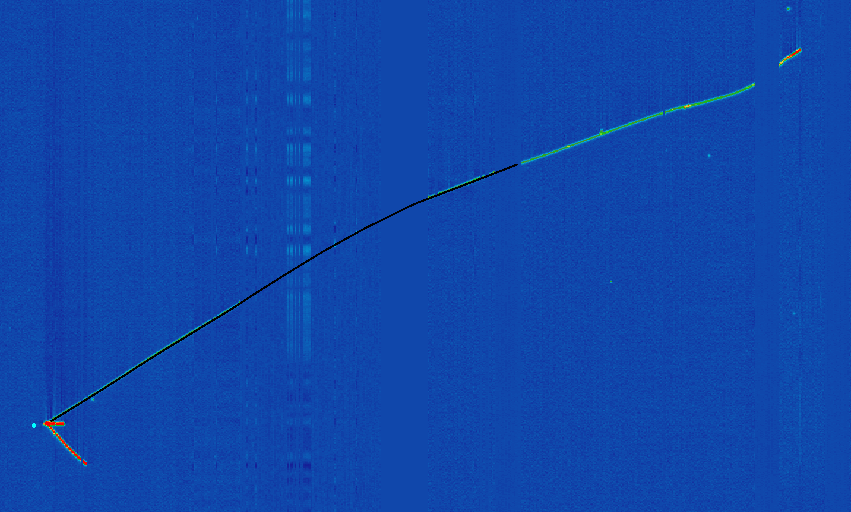
\includegraphics[width=100mm]{Figures/static_figs/bad_evd_1.png}
\end{center}
\caption{\textit{A hand-scanned data event that was deemed ``poorly reconstructed'' and removed from this analysis. The 2D projection of the 3D reconstructed track (shown in black overlaid on raw wire signals) clearly stops before it reaches the end of the particle's trajectory.}}
\label{bad_evd_fig_1}
\end{figure}

\begin{figure}[ht!]
\begin{center}
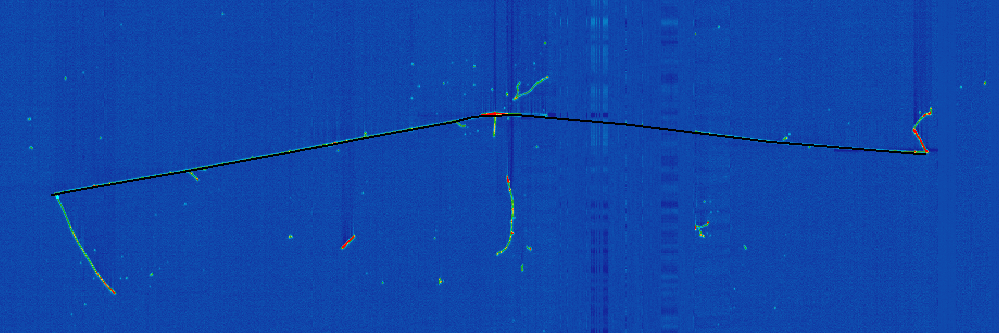
\includegraphics[width=100mm]{Figures/static_figs/bad_evd_2.png}
\end{center}
\caption{\textit{A hand-scanned data event that was deemed some form of MID and removed from this analysis. The 2D projection of the 3D reconstructed track (shown in black overlaid on raw wire signals) matches raw wire signals well, but this event does not appear to be a clean $\nu_\mu$ charged-current event, with at least one neutral pion decay visible near the center of the track.}}
\label{bad_evd_fig_2}
\end{figure}

\begin{figure}[ht!]
\begin{center}
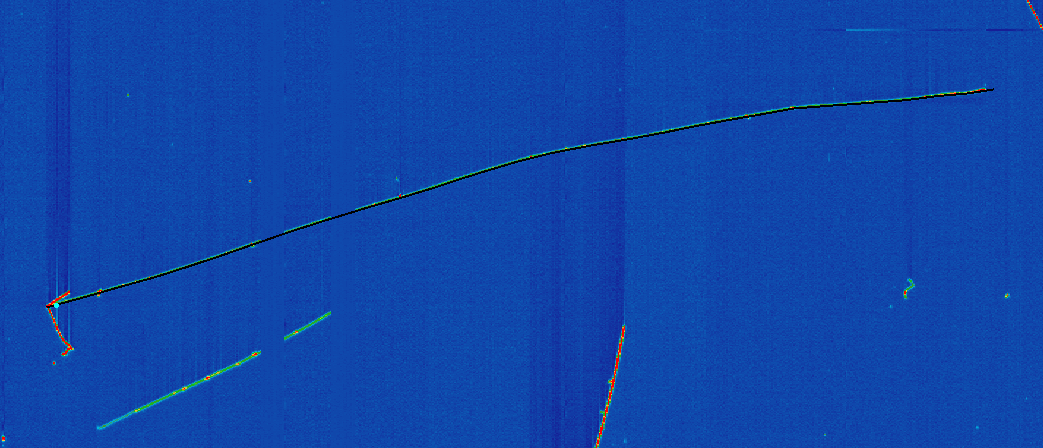
\includegraphics[width=100mm]{Figures/static_figs/good_evd_1.png}
\end{center}
\caption{\textit{A hand-scanned data event that was deemed acceptable for MCS analysis. The track looks well reconstructed, and the wire signals indicate that the particle is likely a muon, and a clear Bragg peak can be seen at the end of the track indicating the track is well contained.}}
\label{good_evd_fig_1}
\end{figure}

\subsection{MCS Momentum Validation}\label{MCS_Momentum_Validation_DataRecoTrack_section}
The MCS momentum versus range-based momentum \textit{without any additional hand-scan reconstruction quality checks} can be seen in Figure \ref{MCS_range_momentum_DataRecoTrack_nohandscan_fig}. The off-diagonal component visible in this figure (where MCS momentum greatly overestimates range momentum) is caused both by poor track reconstruction (truncated tracks) and MIDs. Figure \ref{MCS_range_momentum_RecoTrack_withandwithouthandscan_fig} divides Figure \ref{MCS_range_momentum_DataRecoTrack_nohandscan_fig} into those events which are handscanned as having poorly reconstructed or obviously MID'd tracks, and those which are well reconstructed. It can be seen that hand-scanning tends to remove the off-diagonal component and therefore improve the MCS momentum resolution. Note that only those events which have been hand-scanned as acceptable (Figure \ref{realdata_goodhandscan_fig}) will be used to compute bias and resolutions.\\


The bias and resolution for the MCS momentum estimation method on this sample is computed in the same way as described in previous sections (for example in Section \ref{MCS_Momentum_Validation_MCBNBRecoTrack_section}). The bias and resolution for this momentum reconstruction method is shown in Figure \ref{MCS_range_bias_resolution_MCBNBSelectedRecoTrack_fig}. This figure indicates a bias in the MCS momentum resolution on the order of a few percent, with a resolution that decreases from about 10\% for contained tracks with true total momentum around 0.5 GeV (which corresponds to a length of about 1.7 meters) to below 7\% for contained tracks with true total momentum greater than 0.8 GeV (which corresponds to a length of about 3.1 meters). This agrees well with the analogous plots created from simulated single muons with {\sc MCTracks} (Figure \ref{MCS_range_bias_resolution_MCTrack_fig}).\\

The bias and resolution for this momentum reconstruction method shown in Figure \ref{MCS_range_bias_resolution_DataRecoTrack_fig}. This figure indicates a bias in the MCS momentum resolution on the order of a few percent, with a resolution that decreases from about 10\% for contained reconstructed tracks with range momentum around 0.5 GeV (which corresponds to a length of about 1.7 meters) to about 9\% for contained reconstructed tracks with range momentum greater than 0.8 GeV (which corresponds to a length of about 3.1 meters). This is only slightly higher than the the same bias and resolution measurement in simulation as shown in Figure \ref{MCS_range_bias_resolution_MCBNBSelectedRecoTrack_fig}, a difference which may be attributed to the inefficiencies in hand scanning (as compared to the truth-based MID removal and track-well-reconstructed checks in simulation-based sections). Note the bias and resolution plots here stop at a maximum range-based momentum of below 1.4 GeV due to limited statistics.


\begin{figure}[ht!]
\begin{center}
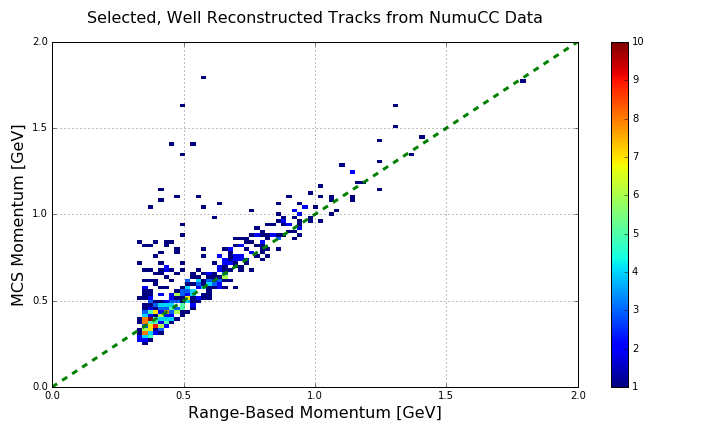
\includegraphics[width=100mm]{Figures/MCS_range_comparison_DataBNBSelectedRecoTrack.png}
\end{center}
\caption{\textit{MCS computed momentum versus range momentum for the selected neutrino-induced fully contained muon sample in data without any additional handscanning to check for reconstruction quality. The off-diagonal where MCS momentum greatly overestimates range momentum is caused by poor track reconstruction (truncated tracks) and MIDs.}}
\label{MCS_range_momentum_DataRecoTrack_nohandscan_fig}
\end{figure}

\begin{figure}
\centering
\mbox{
	\subfigure[\textit{The subset of events in Figure \ref{MCS_range_momentum_DataRecoTrack_nohandscan_fig} which were hand-scanned as having poor reconstruction quality or obvious MID topologies.}]
	{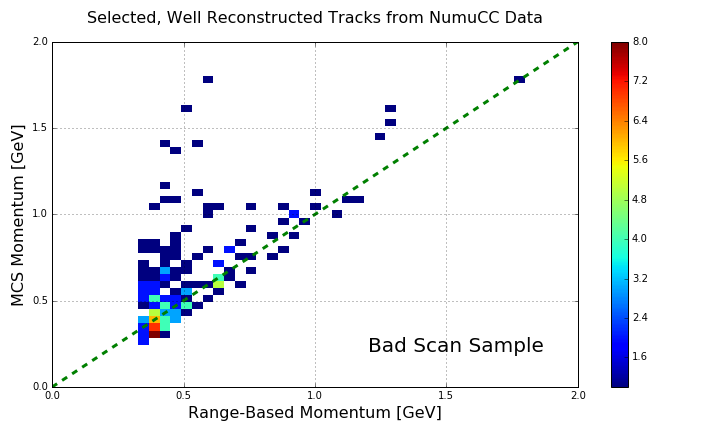
\includegraphics[width=75mm]{Figures/MCS_range_momentum_DataRecoTracks_badhandscan.png}}
	\quad
	\subfigure[\textit{The subset of events in Figure \ref{MCS_range_momentum_DataRecoTrack_nohandscan_fig} which were hand-scanned as having good reconstruction quality or obvious MID topologies.}\label{MCS_range_momentum_DataRecoTrack_fig}\label{realdata_goodhandscan_fig}]
	{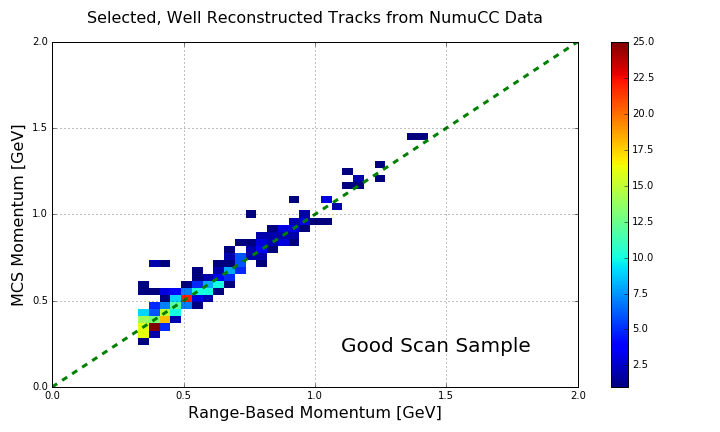
\includegraphics[width=75mm]{Figures/MCS_range_momentum_DataRecoTracks_goodhandscan.png}}
	}
\caption{\textit{MCS computed momentum versus range momentum for the selected neutrino-induced fully contained muon sample in data hand-scanned as having poorly reconstructed tracks (left) and well reconstructed tracks (right).}}
\label{MCS_range_momentum_RecoTrack_withandwithouthandscan_fig}
\end{figure}


\begin{figure}
\centering
\mbox{
	\subfigure[\textit{Fractional momentum difference between 0.35 and 0.53 GeV range momentum.}]
	{\includegraphics[width=75mm]{Figures/{MCS_range_resolution_DataBNBSelectedRecoTrack_slice_0.35_0.53}.png}}
	\quad
	\subfigure[\textit{Fractional momentum difference between 0.90 and 1.08 GeV range momentum.}]
	{\includegraphics[width=75mm]{Figures/{MCS_range_resolution_DataBNBSelectedRecoTrack_slice_0.90_1.08}.png}}
	}
\caption{\textit{Fractional momentum difference for a few representative bins of range momentum derived from Figure \ref{MCS_range_momentum_DataRecoTrack_fig}.}}
\label{MCS_range_bias_resolution_DataRecoTrack_slices_fig}
\end{figure}


\begin{figure}
\centering
\mbox{
	\subfigure[\textit{MCS momentum bias as a function of range momentum. The vertical error bars are computed as $\frac{\sigma_{fit}}{\sqrt{N}}$, and the horizontal error bars indicate bin width.}]
	{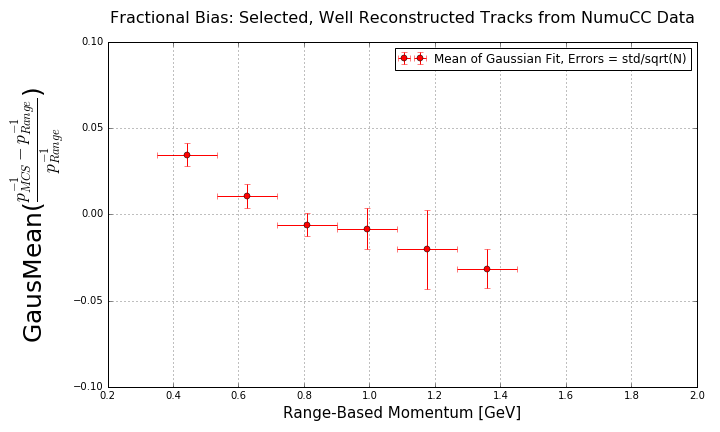
\includegraphics[width=75mm]{Figures/MCS_range_bias_DataBNBSelectedRecoTrack.png}}
	\quad
	\subfigure[\textit{MCS momentum resolution as a function of range momentum. The vertical error bars are computed as $\frac{\sigma_{fit}}{\sqrt{2N}}$, and the horizontal error bars indicate bin width.}]
	{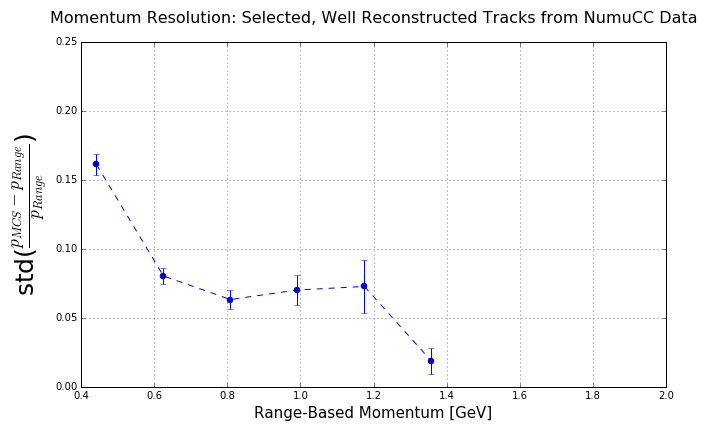
\includegraphics[width=75mm]{Figures/MCS_range_resolution_DataBNBSelectedRecoTrack.png}}
	}
\caption{\textit{MCS momentum bias and resolution as a function of range momentum for the selected, well reconstructed neutrino-induced muons in {\ub} data.}}
\label{MCS_range_bias_resolution_DataRecoTrack_fig}
\end{figure}



\subsection{Highland Validation}\label{Highland_Validation_DataRecoTrack_section}
For this sample of contained, selected, well-reconstructed neutrino-induced tracks in {\ub} data, the same Highland validation plot is created in exactly the same way as described in Section \ref{Highland_Validation_MCTrack_section}. For each consecutive pair of segments, the angular scatter in milliradians divided by the Highland expected RMS in millradians is an entry in the histogram shown in Figure \ref{Highland_validation_DataRecoTracks_fig}. From this figure we can see that the Highland formula is valid for well reconstructed, contained muon tracks in data.

\begin{figure}[ht!]
\begin{center}
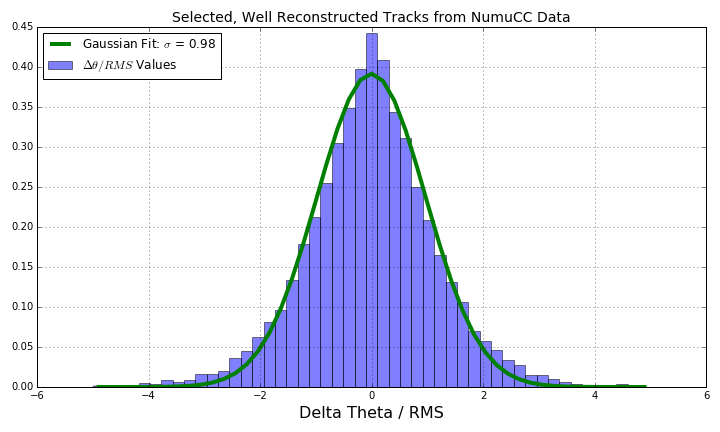
\includegraphics[width=100mm]{Figures/Highland_validation_DataBNBSelectedRecoTrack.png}
\end{center}
\caption{\textit{10 cm segment angular deviations divided by expected Highland RMS for the sample of well reconstructed, neutrino induced muons in {\ub} data.}}
\label{Highland_validation_DataRecoTracks_fig}
\end{figure}











